\chapter{Graphics Support}\label{chapter:Graphics Support}

Graphics support involves having the ability to draw pixels to the screen.\\
Graphics in DaxOS includes:
\begin{itemize}
    \item 1280x720p resolution
    \item Font rendering
    \item Image rendering
\end{itemize}

\section{Enabling Graphics}\label{section:Enabling Graphics}

DaxOS initially used VGA text mode for printing text to the screen. Therefore to get graphics mode, multiboot 
must be configured as follows:

\vspace{0.5cm}
\begin{lstlisting}
    .set FLAGS, ALIGN | MEMINFO | VBEINFO
    .set MODE_TYPE, 0
    .set WIDTH, 1024 
    .set HEIGHT, 768
    .set DEPTH, 32
\end{lstlisting}
\pagebreak

The \textbf{MODE\_TYPE} indicates that we want to be able to draw pixels instead of text and \textbf{depth} indicates
that each pixel requires 32 bits for representation. Thus each pixel follows the ARGB form where:
\begin{itemize}
    \item A is alpha transparency.
    \item R, G and B are red, green and blue components respectively.
\end{itemize}

Now we can draw pixels to the screen by writing to the framebuffer address.


\section{Font Rendering}\label{section:Font Rendering}

With VGA text-mode, the complexity of rendering fonts were handled by the BIOS. However, in graphics mode, DaxOS must
implement its own font renderer. The idea here is that in order to print a letter to the screen, a bitmap of the 
letter must be generated from the font and it must be copied into the framebuffer.

The sequence of steps to be followed to get the font bitmap is as follows:
\begin{itemize}
    \item Choose any bitmap based font.
    \item Convert the font to .ssfn format.
    \item Convert the .ssfn file into object file.
    \item Link the font file with the OS. 
\end{itemize}

To render fonts to the screen DaxOS uses a modified verson of a font renderer called scalable screen font renderer.
The modifications introduced include:
\begin{itemize}
    \item Refactoring to split ssfn.h into corresponding .h and .c file.
    \item Removing unwanted functionality from the source.
\end{itemize}

\pagebreak
\section{Image Rendering}\label{section:Image Rendering}
DaxOS support rendering images in Truevision TGA format. The image is converted to .tga format and linked with the OS as described
previously.
Rendering images is then a two step process:
\begin{itemize}
    \item Decode the TGA header to get the image metadata.
    \item Iterate and copy pixel data of image to framebuffer.
\end{itemize}

The tga header is as follows:
\begin{lstlisting}
    typedef struct
    {
        unsigned char magic1;             // must be zero
        unsigned char colormap;           // must be zero
        unsigned char encoding;           // must be 2
        unsigned short cmaporig, cmaplen; // must be zero
        unsigned char cmapent;            // must be zero
        unsigned short x;                 // must be zero
        unsigned short y;                 // image's height
        unsigned short w;                 // image's width
        unsigned short h;                 // image's height
        unsigned char bpp;                // must be 32
        unsigned char pixeltype;          // must be 40
    } __attribute__((packed)) tga_header_t;
\end{lstlisting}

Of all the fields, the image width and height are most important. This header is located at the start of the image.
Therefore skipping over this header gives the pixel data of the image. 
Copying pixel data to the framebuffer is then done using memcpy function.

\begin{figure}[h!]
	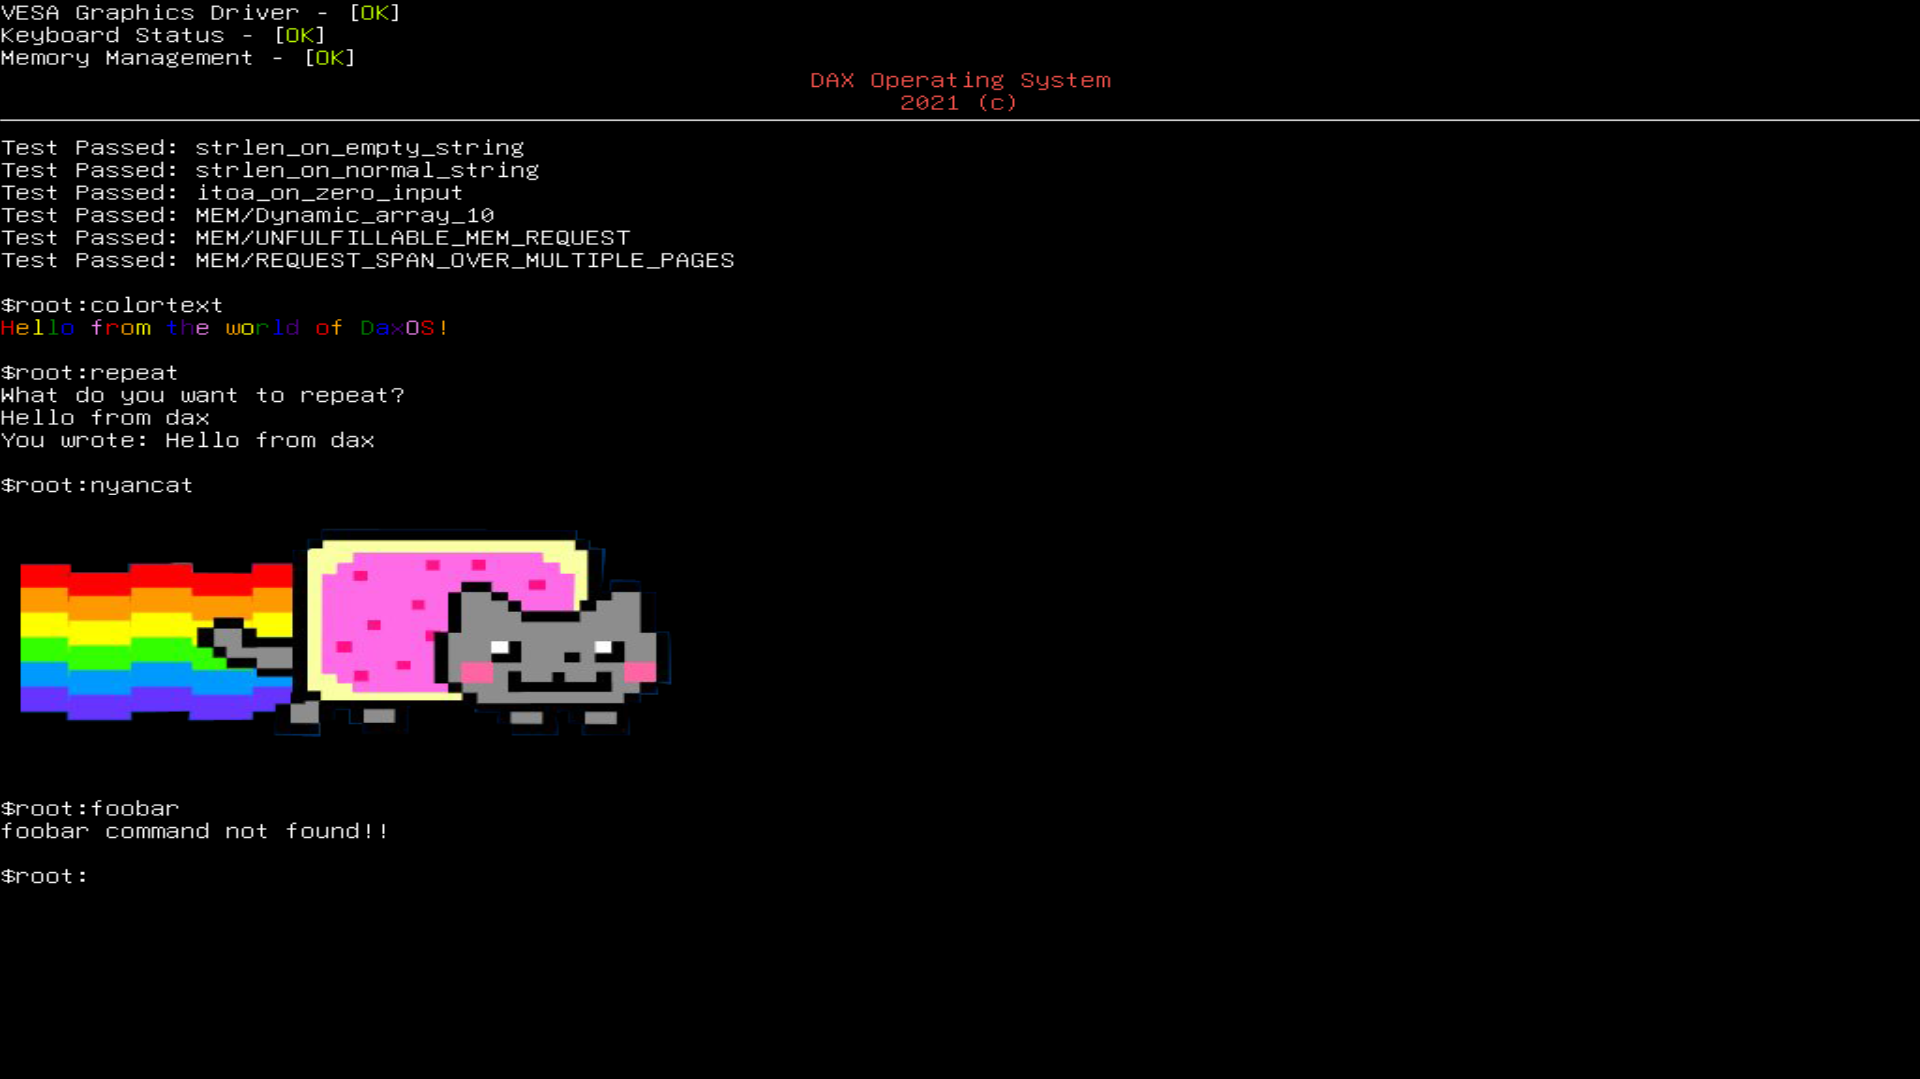
\includegraphics[width=\textwidth,height=\textheight,keepaspectratio]{image}
	\caption{Image rendering in DaxOS}
\end{figure}
\clearpage